\documentclass[12pt]{article}

% PAQUETES
\usepackage[headheight=20pt, headsep=1cm, margin=1in]{geometry} % <-- este es el cambio clave
\usepackage{graphicx}
\usepackage{booktabs}
\usepackage{amsmath, amssymb}
\usepackage{threeparttable}
\usepackage{fancyhdr}
\usepackage{caption}
\usepackage{lmodern}
\usepackage{multicol}
\usepackage{tabularx}
\usepackage{float}

% ENCABEZADO PERSONALIZADO
\pagestyle{fancy}
\fancyhf{}
\lhead{\includegraphics[height=1.5cm]{logo.png}}
\cfoot{\thepage}


\begin{document}

\begin{center}
    \vspace*{1cm}
    \Large \textbf{Third assignment - CTA200H Course} \\[0.5cm]
    \large Juan Carlos Aranda Muñoz \\[0.2cm]
    \normalsize May 2025
    \vspace{1cm}
\end{center}
\renewcommand{\arraystretch}{1.2} % extra space between rows

\section{Exercise: Mandelbrot Set}

\subsection*{Method}
To visualize the Mandelbrot set, we numerically iterated the complex function:
\[
z_{n+1} = z_n^2 + c, \quad z_0 = 0
\]
for each point \( c = x + iy \) on a dense grid of the complex plane, specifically over the region \( -2 < x < 2 \), \( -2 < y < 2 \). The key idea is that some values of \( c \) will generate sequences \( \{z_n\} \) that remain bounded (i.e., never exceed a magnitude of 2), while others will diverge to infinity.

The code used a resolution of 800×800 points, creating a grid of complex numbers using:
\begin{verbatim}
C = x[np.newaxis, :] + 1j * y[:, np.newaxis]
\end{verbatim}
We wrote a custom function \texttt{iteration(c, max\_iter)} (in a separate Python module) that:
\begin{enumerate}
    \item Sets \( z_0 = 0 \)
    \item Iteratively computes \( z_{n+1} = z_n^2 + c \)
    \item Stops and returns the iteration count \( n \) if \( |z_n| > 2 \)
    \item Returns \texttt{max\_iter} if the value stays bounded within the limit
\end{enumerate}

\noindent Two 2D arrays were created:
\begin{itemize}
    \item \texttt{divergence[i, j]}: records how many iterations it took to escape for each point \( c \)
    \item \texttt{mask[i, j]}: records whether each point remained bounded (i.e., if it survived all \texttt{max\_iter} steps)
\end{itemize}

\subsection*{Result and Analysis}
The first plot shows the classical Mandelbrot set: bounded points are rendered in black, and those that diverge are in white.

\begin{figure}[H]
    \centering
    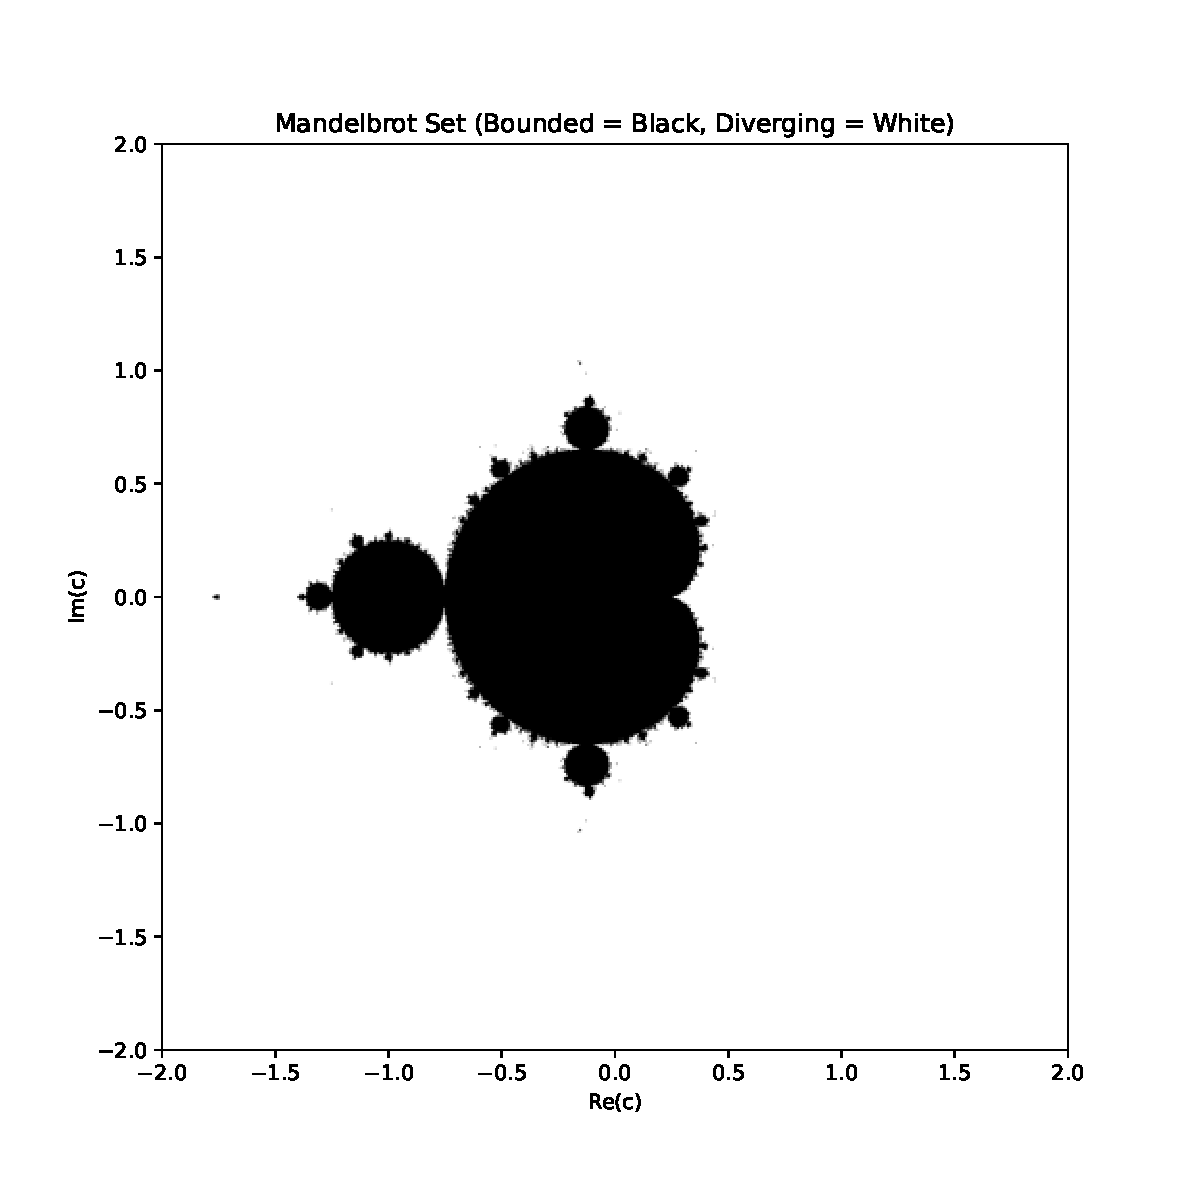
\includegraphics[width=0.7\textwidth]{mandelbrot_1.pdf}
    \caption{Mandelbrot set: black = bounded points, white = diverging points.}
\end{figure}

We observe that the Mandelbrot set is a highly structured fractal: the main cardioid and surrounding bulbs represent the values of \( c \) where the iterative function is stable. These are regions where the orbit of \( z_n \) remains bounded, giving rise to self-similar and intricate boundary detail upon magnification.

The second plot provides deeper insight by using a color map (`plasma`) to visualize the \emph{escape time} — the number of iterations it took for \( z_n \) to exceed a magnitude of 2.

\begin{figure}[H]
    \centering
    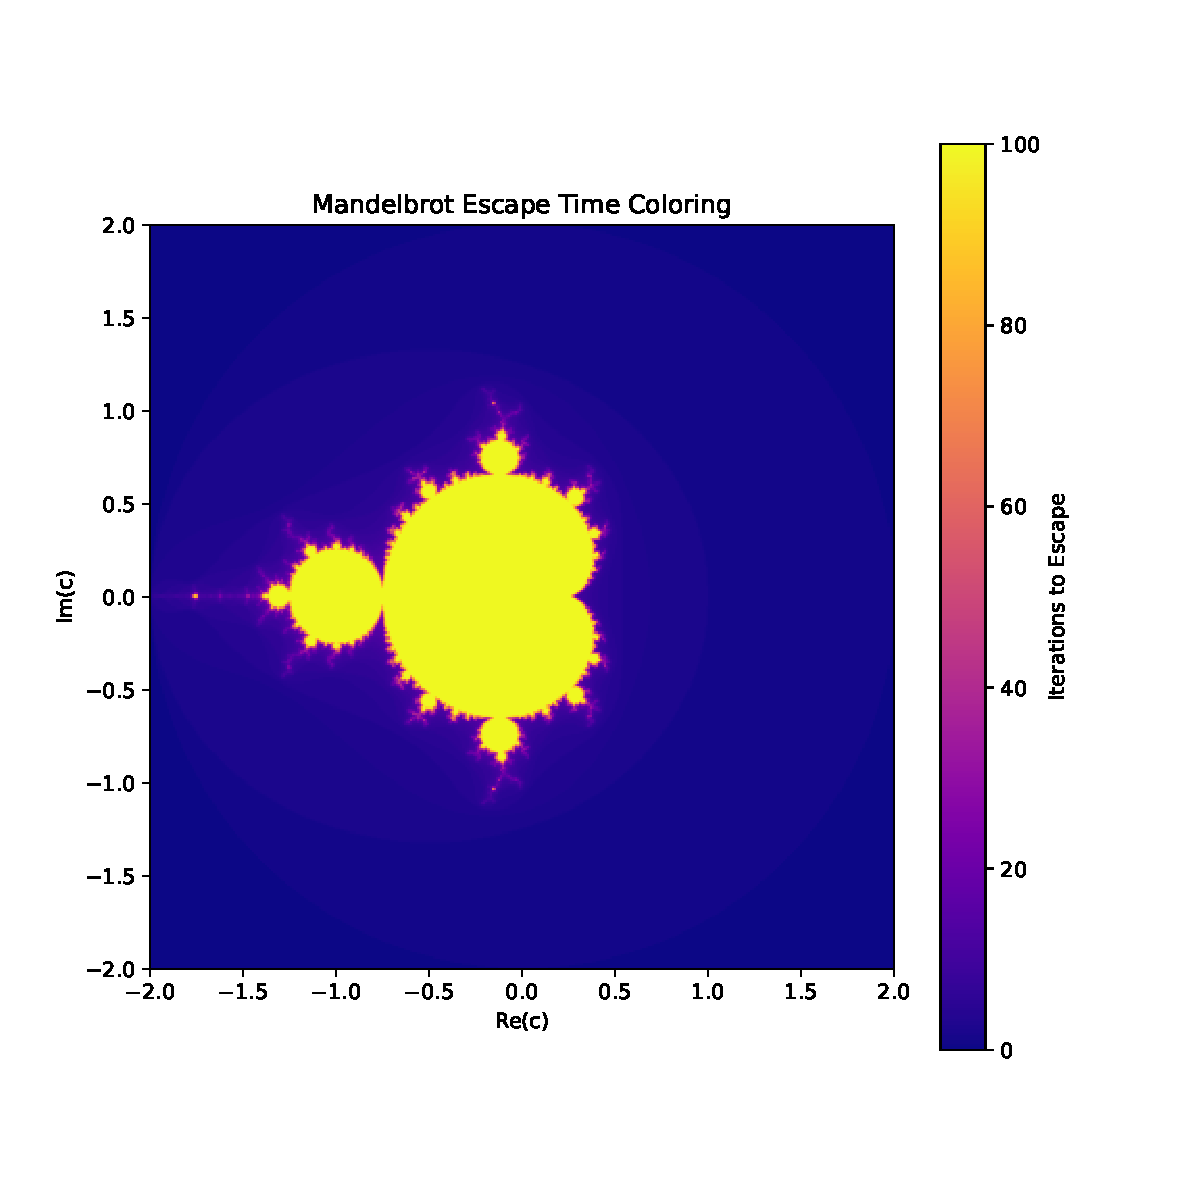
\includegraphics[width=0.7\textwidth]{mandelbrot_2.pdf}
    \caption{Escape time coloring: brighter colors indicate slower divergence.}
\end{figure}

This color-coded version reveals more about the rate of divergence. Points closer to the boundary of the Mandelbrot set take longer to escape, creating a halo of slow-diverging points. This provides both mathematical and visual intuition: near the edge, the function is highly sensitive, and even tiny changes in \( c \) can dramatically change the behavior of the orbit. This is a hallmark of fractal and chaotic systems.

We used a maximum of 100 iterations. Increasing this number yields finer boundaries but increases computational time. For higher-quality renders, a trade-off between resolution and iteration depth is necessary.


\section{Exercise: The Lorenz Model}

\subsection*{Method}
This exercise implements the classical Lorenz system of differential equations:
\[
\begin{aligned}
\frac{dX}{dt} &= \sigma (Y - X), \\
\frac{dY}{dt} &= rX - Y - XZ, \\
\frac{dZ}{dt} &= XY - bZ,
\end{aligned}
\]
which models convective fluid flow and exhibits chaotic behavior under certain parameters. We coded the system as a Python function using proper docstrings for clarity. The "scipy.integrate.solve\_ivp" routine was used to numerically integrate the system from \( t = 0 \) to \( t = 60 \) (in dimensionless time units), using initial conditions \( W_0 = [0, 1, 0] \) and the canonical parameters \( (\sigma, r, b) = (10, 28, 8/3) \).

A fixed time step of \( \Delta t = 0.01 \) was used for evaluation, matching the one used in Lorenz's original 1963 paper. We used a high-precision integrator with strict tolerances (\texttt{rtol} and \texttt{atol} set to \( 10^{-10} \)) to faithfully reproduce the sensitive dependence on initial conditions.

\subsection*{Results and Analysis}

\subsubsection*{Reproduction of Lorenz Figure 1}

The first set of plots displays the evolution of the \( Y \) variable over three consecutive windows of 1000 iterations each. The x-axis corresponds to the iteration number \( N = t / \Delta t \).

\begin{figure}[H]
    \centering
    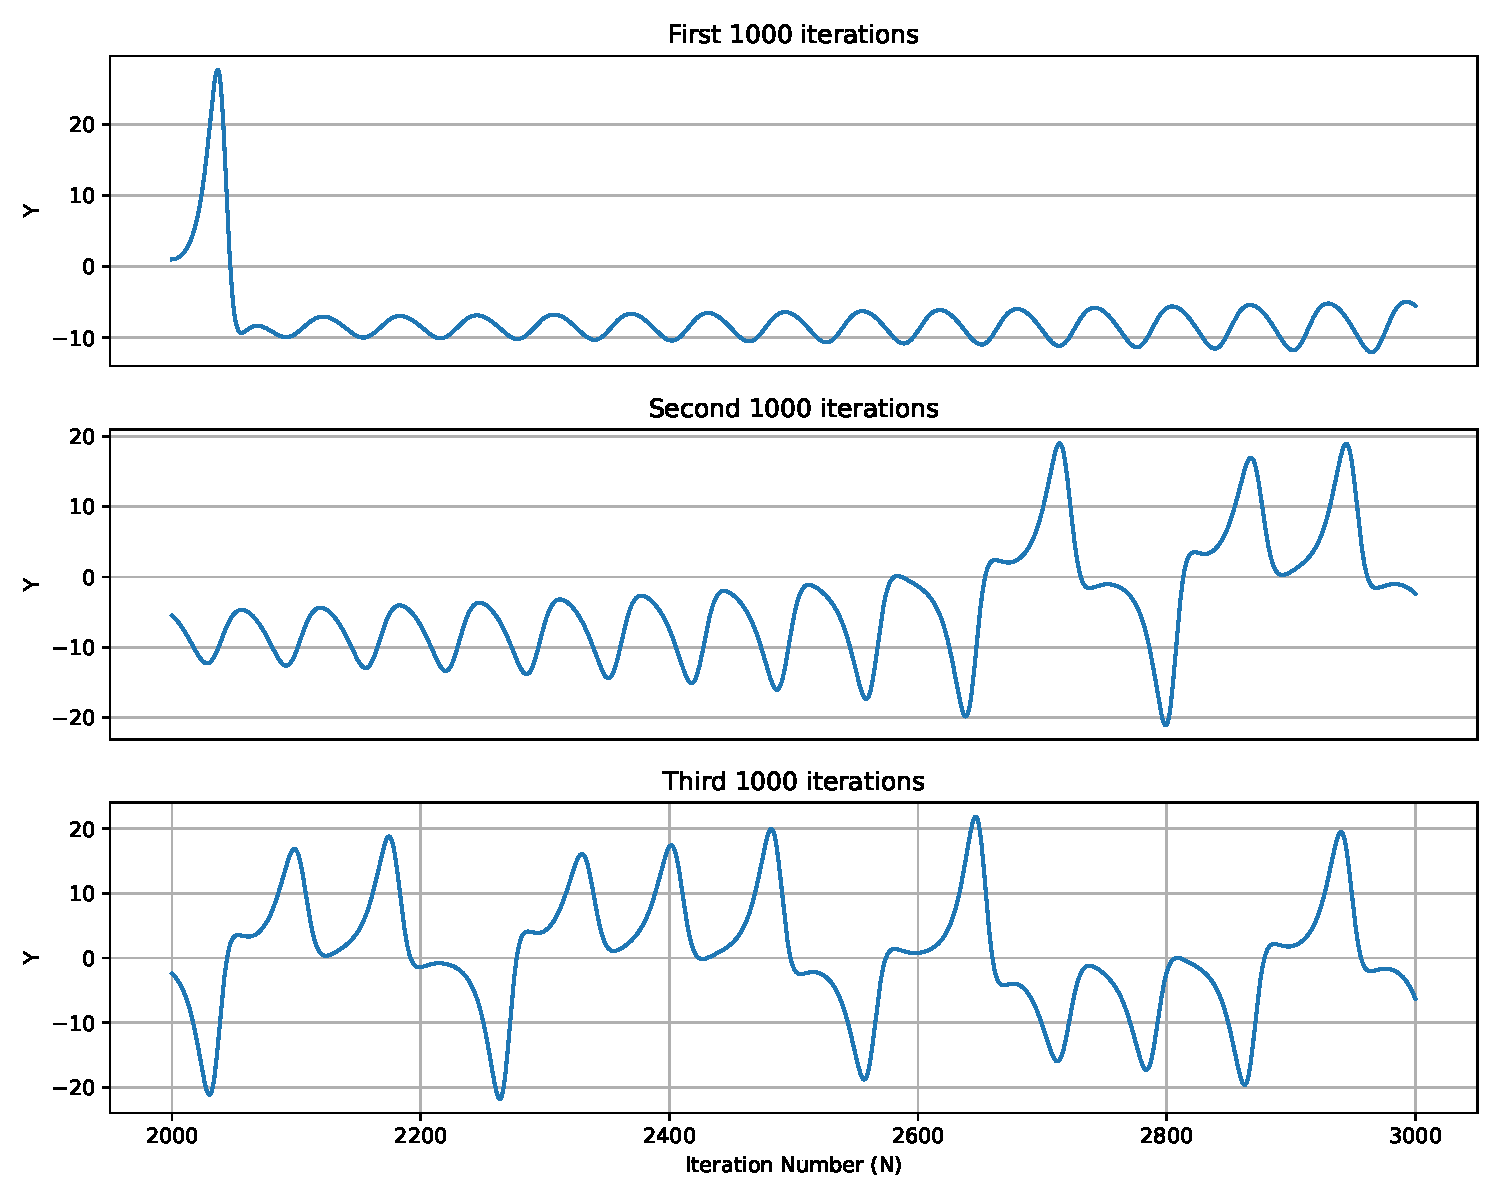
\includegraphics[width=\textwidth]{lorenz_figure1.pdf}
    \caption{Reproduction of Lorenz's Figure 1: $Y$ vs iteration number $N$, for three 1000-step intervals.}
\end{figure}

The chaotic nature of the system is evident — even though the system is deterministic, it does not settle into a fixed point or periodic orbit. Instead, the trajectory exhibits oscillations of varying amplitude and apparent unpredictability, even within these relatively short time windows.

\subsubsection*{Reproduction of Lorenz Figure 2}

We then reproduced Lorenz's Figure 2 by projecting the solution in two ways:
\begin{itemize}
    \item Top: a $Y$-$Z$ projection from iteration 1400 to 1900.
    \item Bottom: a $Y$-$X$ projection (with inverted Y-axis) over the same interval.
\end{itemize}
Both subplots are annotated with numerical time labels (e.g., '14' for the positions at the \( iteration=1400 \), etc.) to match the original paper.

\begin{figure}[H]
    \centering
    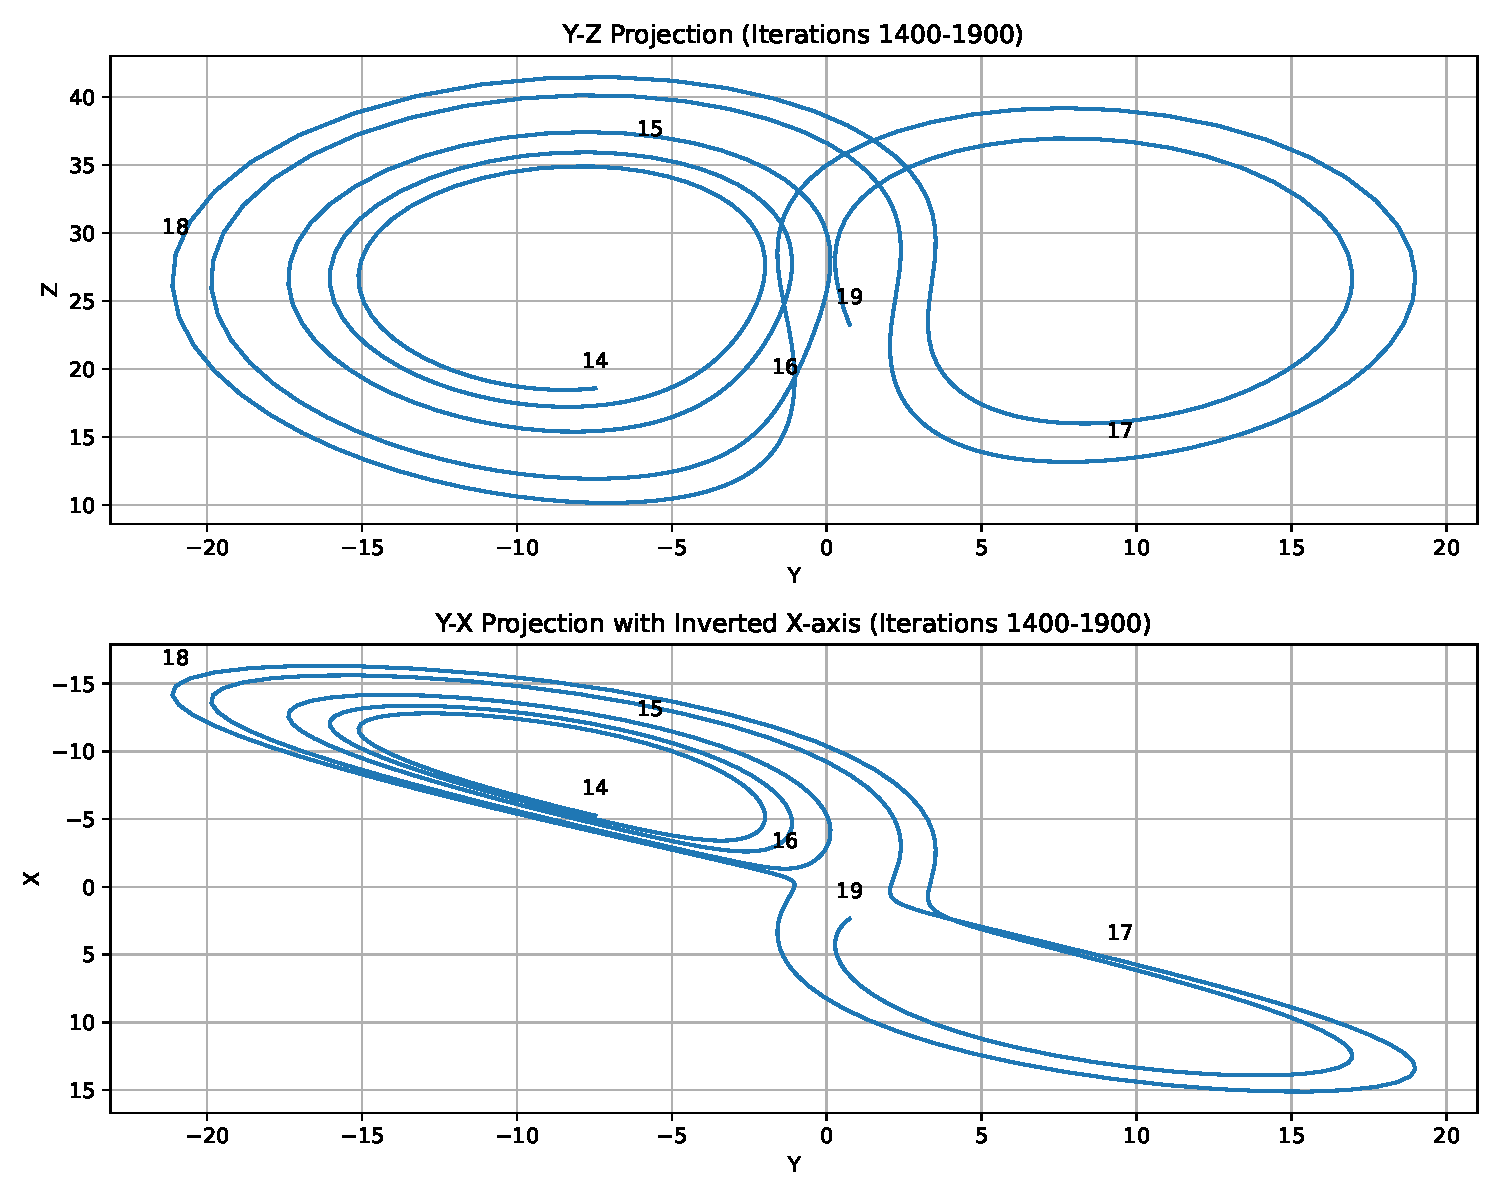
\includegraphics[width=\textwidth]{lorenz_figure2.pdf}
    \caption{Reproduction of Lorenz's Figure 2: Top — $Y$ vs $Z$; Bottom — $Y$ vs $X$ with inverted axis, labeled with $t$ in dimensionless units.}
\end{figure}

These projections illustrate how the solution evolves through the "butterfly" attractor structure. Despite never repeating exactly, the trajectory remains confined to a bounded region of phase space.

\subsubsection*{Sensitivity to Initial Conditions}

Finally, to quantify the system's sensitive dependence on initial conditions, we ran a second simulation with a tiny perturbation in the initial condition: \( W_0' = [0, 1.00000001, 0] \). We computed the Euclidean distance between the original and perturbed trajectories at each time point.

\begin{figure}[H]
    \centering
    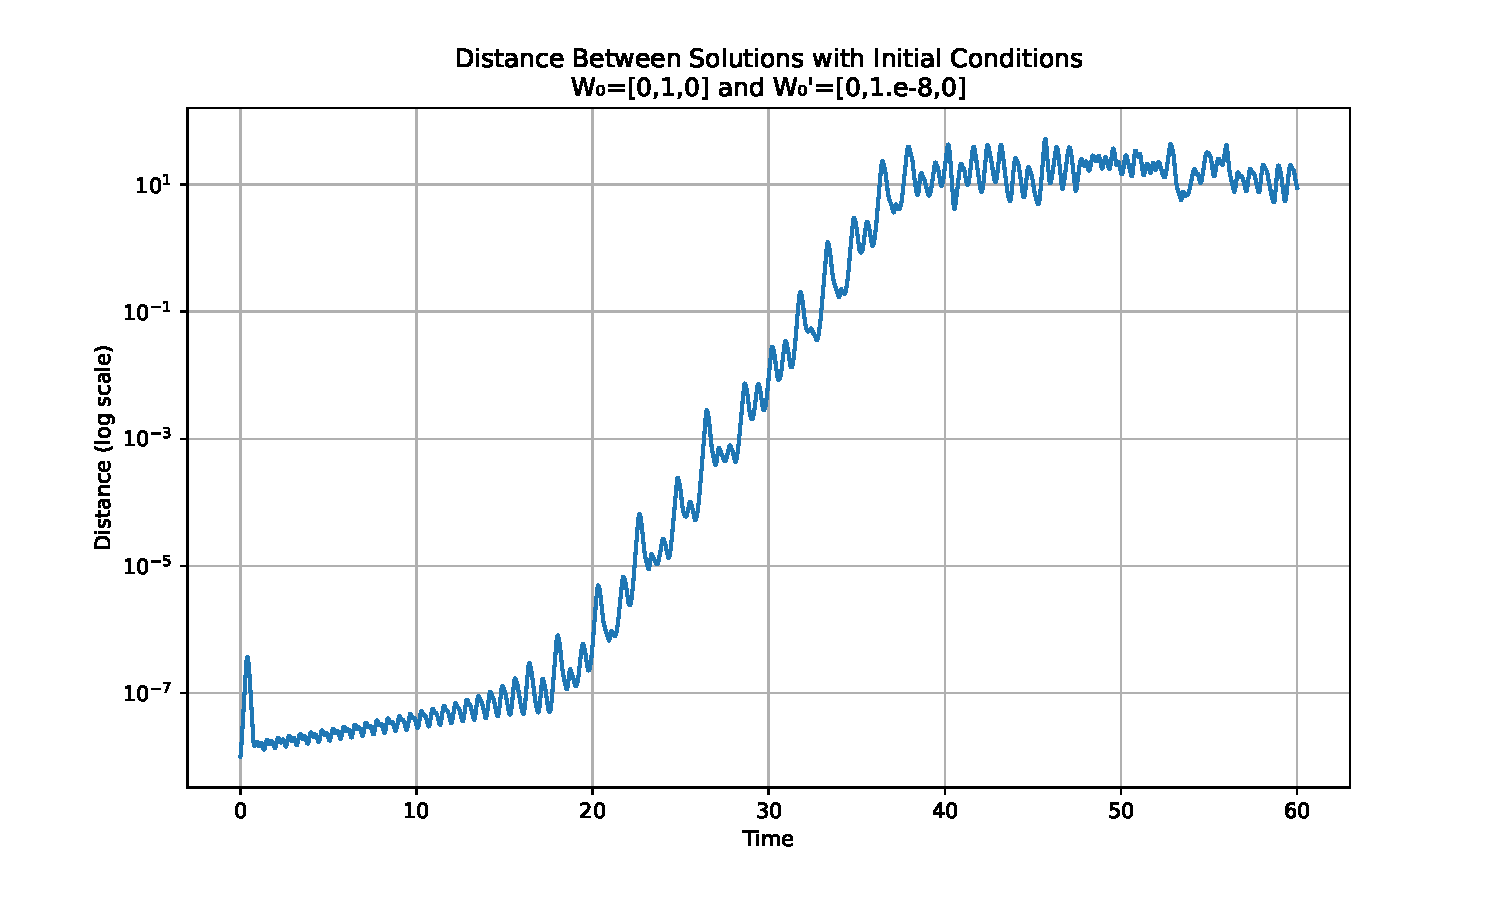
\includegraphics[width=0.8\textwidth]{lorenz_sensitivity.pdf}
    \caption{Growth of distance between solutions with initial conditions $W_0$ and $W_0'$. The semilog plot reveals exponential divergence.}
\end{figure}

The distance grows exponentially with time, appearing as a straight line in a semilog plot. This is direct evidence of the butterfly effect: tiny differences in starting points rapidly amplify, making long-term predictions practically impossible. This behavior is what originally led Lorenz to question the predictability of weather and led to foundational insights in chaos theory.


\end{document}
